\documentclass[11pt]{article}

% --- page and typography ---
\usepackage[a4paper,margin=1in]{geometry}
\usepackage{microtype}
\usepackage[T1]{fontenc}
\usepackage{lmodern}
\linespread{1.05}

% --- math, units, figures, tables ---
\usepackage{amsmath}
\usepackage{siunitx}
\sisetup{detect-all, range-phrase={\text{--}}, range-units=single}
\usepackage{graphicx}
\graphicspath{{../figures/}}
\usepackage{booktabs}
\usepackage[font=small,labelfont=bf]{caption}
\usepackage{placeins}

% --- references ---
\usepackage[backend=biber,style=numeric-comp,sorting=none,giveninits=true,maxbibnames=8,doi=true,url=false,isbn=false]{biblatex}
\addbibresource{references.bib}

% --- links and cross-refs (load hyperref then cleveref last) ---
\usepackage[hidelinks]{hyperref}
\usepackage[capitalise,nameinlink]{cleveref}

% Reusable notation. Keep small; do not over-abstract.
\newcommand{\LD}{\textit{L/D}}
\newcommand{\ms}{\,\unit{\meter\per\second}}
\newcommand{\degr}{^{\circ}}
\newcommand{\cgfrac}{x_\mathrm{cg}}
\newcommand{\npfrac}{x_\mathrm{np}}


\title{\bfseries Wind, slope, and the want of a tail:\\
a computational feasibility study of Eilmer of Malmesbury's flight}

% Author block per ~/dev/Rules/AUTHORSHIP.md. Interface uses single-anonymized
% review, so the named block is the default; \def\anon{} produces a blind build.
\ifdefined\anon
  \author{}
\else
  \author{David H. Silver \\[3pt]
    {\normalsize Remiza, Poughkeepsie, NY, USA} \\[1pt]
    {\small \texttt{david@remiza.ai} \,\textperiodcentered\, ORCID 0000-0002-3071-304X}}
\fi
\date{}

\begin{document}
\maketitle

\begin{abstract}
\noindent
Around 1000--1045 a monk at Malmesbury Abbey fixed wings to his hands and feet,
glided from a tower for ``more than a furlong'' (about \SI{200}{\meter}), crashed,
broke both legs, and blamed the failure on having no tail.
We test that account as a constrained engineering problem using terrain
reconstruction, twenty years of ERA5 wind climatology, a first-order ridge-lift
model, a glide-and-stability analysis, a 40,000-sample Monte Carlo over the unknown
apparatus, and an impact-biomechanics model.
The abbey sits on a SW-facing escarpment aligned with the prevailing wind, which is
favourable for launch in \SI{15.6}{\percent} of hours per year.
A still-air glide would demand a sailplane-class glide ratio of \num{11.1}, but
ridge lift over the escarpment brings the requirement within reach of a crude
cambered wing (\LD\ \numrange{3}{7}) above roughly \SI{3.6}{\meter\per\second} of
wind.
A tailless hand-and-foot wing is statically unstable across every centre of gravity
a hanging pilot can reach, and its pitch error doubles in a median \SI{0.27}{\second}
against a flight lasting some \SI{20}{\second}; adding a tail removes the divergence.
The predicted out-of-control arrival breaks both legs yet remains survivable,
matching the reported injury.
The account is internally consistent and Eilmer's own diagnosis is correct.
We release the full pipeline so the method can adjudicate other pre-modern flight
claims.
\end{abstract}

\section{Introduction}

In the eleventh century a monk of Malmesbury Abbey named Eilmer fixed wings to his
hands and feet, leapt from a tower, glided for ``more than a furlong,'' and crashed,
breaking both legs and walking lame for the rest of his life.
He later said the fault was his own: he had fitted no tail.
This paper asks whether that account is physically self-consistent, and finds that
it is.
A wind-and-slope-assisted glide of about \SI{200}{\meter} from the abbey is
feasible for a crude cambered wing; a tailless hand-and-foot apparatus is
statically unstable for any pilot posture and loses pitch control within a second
of a disturbance; and the resulting out-of-control impact breaks both legs while
remaining survivable.
Eilmer's own diagnosis, the want of a tail, is the correct one.

The source is good by the standards of medieval history.
William of Malmesbury, writing about a century later in the same house, knew men who
had known Eilmer, and records concrete and testable details: a tower launch, wings
on the hands and feet, a breeze, a glide of a furlong, a fall, broken legs, and the
missing tail \autocite{williamMalmesbury_gesta,white1961eilmer}.
Each of these is an engineering constraint.
The question is not whether a medieval monk \emph{could have} understood
aerodynamics, but whether the event he is reported to have survived is consistent
with the aerodynamics we understand now.

\begin{figure}[htbp]
  \centering
  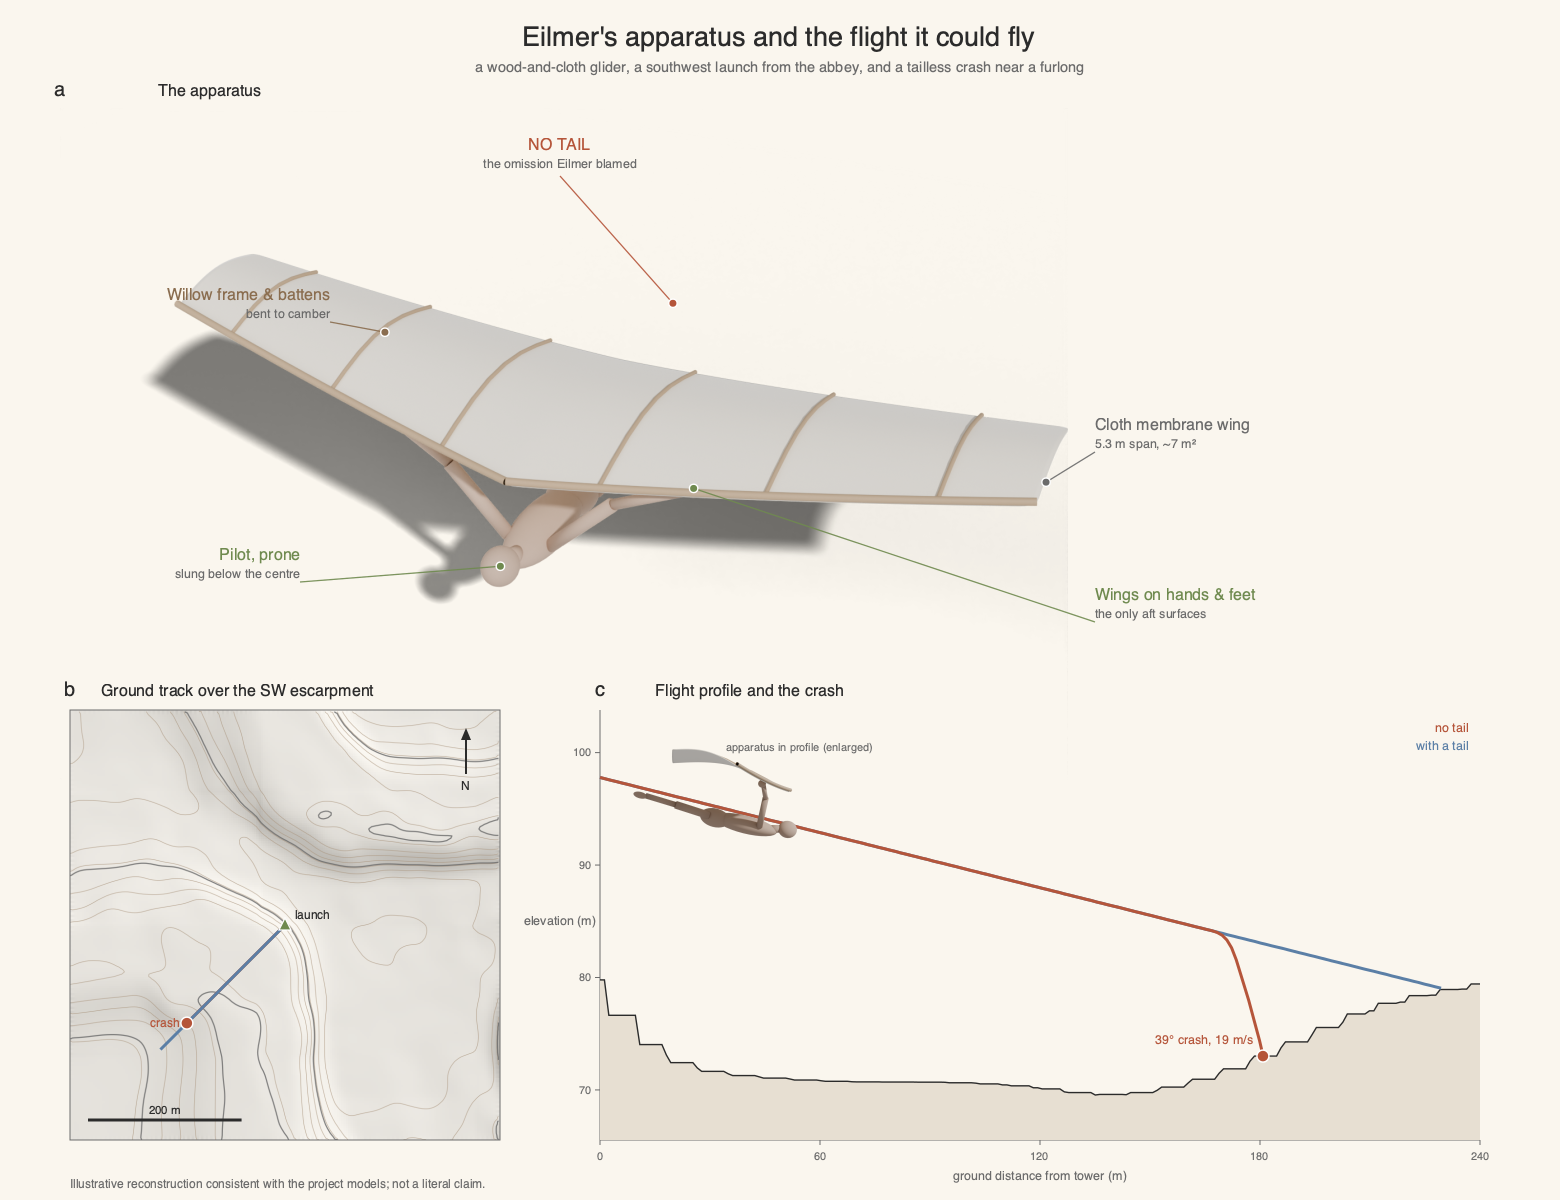
\includegraphics[width=\linewidth]{apparatus_flight.png}
  \caption{\textbf{Eilmer's apparatus and the flight it could fly.}
  \textbf{(a)} A to-scale reconstruction of the apparatus implied by the glide and
  stability models: a cambered cloth-membrane wing of about \SI{7}{\meter\squared}
  and \SI{5.3}{\meter} span (aspect ratio 4) on a willow frame, the pilot prone with
  wings fixed to the hands and feet and, as William of Malmesbury records, no tail.
  \textbf{(b)} Launch geometry on the abbey promontory, with the southwest ground
  track of the glide over a contour map of the escarpment, from the tower to an
  impact about a furlong away.
  \textbf{(c)} The flight in profile, apparatus enlarged for clarity: a
  wind-and-slope-assisted glide with a tail (blue) against the tailless case (red),
  which loses pitch control and strikes the ground at about \ang{39} and
  \SI{19}{\meter\per\second}.
  The reconstruction is illustrative and consistent with the project models, not a
  literal depiction.}
  \label{fig:apparatus}
\end{figure}

We treat the flight as a constrained engineering problem and attack it with the
tools available in 2026: a digital terrain model of the abbey promontory, two
decades of reanalysis wind climatology, a first-order orographic lift model, a
glide and short-period pitch-stability analysis, a Monte Carlo over the unknown
apparatus geometry and launch day, and an impact-biomechanics model calibrated to
human long-bone fracture tolerances.
\Cref{fig:apparatus} summarises the reconstruction and the result.
The contribution is twofold: a calibrated verdict on a specific historical claim,
and a reproducible method for adjudicating pre-modern flight accounts from terrain,
climate, and first-principles flight dynamics rather than from anecdote.
Everything here rebuilds from raw data with a single command, and the apparatus we
infer is a consequence of the models, not an input to them.

\section{The source, the date, and prior work}

William of Malmesbury reports the flight in his \textit{Gesta Regum Anglorum}
(about 1125), within living memory of the abbey's older monks and roughly a century
after the event \autocite{williamMalmesbury_gesta}.
He names Eilmer, describes the apparatus as wings on the hands and feet, gives the
distance as more than a stadium (a furlong, about \SI{200}{\meter}), reports that
wind or turbulence and his own fear brought him down, and that he broke both legs.
He adds Eilmer's retrospective explanation that he had forgotten to fit a tail.
This is the canonical account, and Lynn White's study remains the standard
historical treatment \autocite{white1961eilmer}; later popular and survey histories
follow it \autocite{hallion2003takingflight,scott1995shoulders,lacey2004greattales},
and the \textit{Oxford Dictionary of National Biography} dates Eilmer to about
985 and after 1066 \autocite{thomson2004eilmer_odnb}.

The date of the flight is an open and actively debated question.
The traditional reconstruction ties Eilmer's later comet sighting to the returns of
Halley's comet and places the flight around 1000--1010
\autocite{woosnam1986eilmer,lewispz_bayeuxcomet}.
\textcite{aitcheson2026date}, writing this year in \textit{Notes and Queries},
reopens it: the earlier comet Eilmer recalled may have been the comet of 1018 rather
than the 989 apparition of Halley, which would move his birth into the 990s to 1010s
and the flight itself as late as the 1020s, 1030s, or early 1040s, decades later than
the standard date.
The window is therefore wider and less settled than the textbooks imply, and we do
not try to close it.
Because the flight depends on weather rather than on the calendar year, we treat the
launch day as a variable sampled from the wind climatology of the site
(\cref{sec:results}).
That choice makes our analysis insensitive to the dating dispute: the relevant
prevailing-wind regime is stable across the whole eleventh-century window Aitcheson
admits, so the feasibility verdict holds whichever decade the leap belongs to.

Human-flight attempts before the modern era are mostly legend, and the
historiography is careful to separate reportable fact from myth-making
\autocite{paz2013humanflight}.
Eilmer is unusual in having a credible near-contemporary witness and a named,
physical cause of failure.
The closest antecedent is the ninth-century Andalusian polymath Abbas Ibn Firnas,
who is reported to have glided and likewise landed badly, traditionally also blamed
on the lack of a tail \autocite{anderson2024bridge}.
That two of the earliest credible accounts converge on the same aerodynamic
diagnosis is itself worth a quantitative test.
The name of the modern open-source hypersonic flow solver \textit{Eilmer} honours
this same monk \autocite{gibbons2022eilmer,jacobs2017eilmer4}, a small reminder that
the aerodynamics community already claims him.

\section{Methods}
\label{sec:methods}

The analysis is split into independent workstreams, each writing a
\texttt{metrics.json} that feeds both its figure and the numbers quoted here, so a
single source produces every value.
The whole pipeline rebuilds from raw data with one driver script.

\subsection{Terrain}

We build a digital elevation model of the abbey promontory from AWS Terrain Tiles
(terrarium encoding, zoom 14, about \SI{6}{\meter} posting).
From it we compute the local slope and aspect within a \SI{400}{\meter} radius of
the tower and extract an elevation section along the dominant SW--NE axis.
The \SI{6}{\meter} posting under-resolves the sharp launch edge, so slope estimates
are reported as lower bounds pending airborne LIDAR.

\subsection{Wind climatology}

We take twenty years of ERA5 hourly \SI{10}{\meter} wind at the abbey (2004--2023,
\num{175320} hours) through the Open-Meteo archive
\autocite{hersbach2020era5,openmeteo_archive}.
A launch is counted favourable when the wind lies in the SW sector
(\ang{191}--\ang{259}, aligned with the escarpment aspect) at \SIrange{5}{12}{\meter\per\second}.
We report the favourable fraction annually and by meteorological season with
\SI{95}{\percent} confidence intervals taken across the twenty years.
Reconstructions of the medieval North Atlantic Oscillation differ on timing,
from a persistently positive Medieval Climate Anomaly mode
\autocite{trouet2009nao} to one with positive phases concentrated in later centuries
\autocite{ortega2015nao}, but neither points to the weak westerlies of a negative
phase, so modern reanalysis is a reasonable and probably conservative proxy
for Eilmer's epoch; the Twentieth Century Reanalysis provides an independent
stationarity check \autocite{slivinski2019twentieth}.

\subsection{Ridge lift}

We model orographic lift over the real terrain section with a first-order linear
solution in which the vertical air velocity follows the surface slope and decays
with height,
\begin{equation}
  w(x,z) = U\,\frac{\mathrm{d}h}{\mathrm{d}x}\,e^{-kz},
  \label{eq:ridge}
\end{equation}
where \(U\) is the incoming wind speed, \(\mathrm{d}h/\mathrm{d}x\) the along-wind
surface slope, \(z\) height above the surface, and \(k = 2\pi/L\) a decay rate set
by the escarpment horizontal scale \(L\).
We compare the resulting lift against a crude glider's sink rate to estimate the
depth of the soarable band.
\Cref{eq:ridge} is a deliberately conservative stand-in for a microscale large-eddy
or WAsP solve, which is deferred to a LIDAR-resolved follow-up.

\subsection{Glide}

Steady gliding flight sets the airspeed and sink rate.
For mass \(m\), wing area \(S\), trim lift coefficient \(C_L\), and air density
\(\rho\), the trim airspeed is \(V = \sqrt{2mg/(\rho S C_L)}\), the glide angle
\(\gamma\) satisfies \(\tan\gamma = 1/(\LD)\), and the still-air sink is
\(V\sin\gamma\).
With orographic upwash \(w\) the net sink is \(V\sin\gamma - w\), and the ground
range from launch height \(h\) is \(R = V\cos\gamma \cdot h/\max(V\sin\gamma-w,\,0)\),
extended without limit where the net sink is non-positive (the pilot soars).
We invert \(R = \SI{200}{\meter}\) to find the glide ratio required as a function of
wind speed, and compare it against the crude cambered-wing band (\LD\
\numrange{3}{7}) supported by low-Reynolds-number airfoil data
\autocite{lissaman1983lowre,hoerner1985lift,drela2014flight,faa_glider}.

\subsection{Pitch stability}

Longitudinal stability turns on the centre of gravity \(\cgfrac\) relative to the
neutral point \(\npfrac\), both in fractions of the mean chord.
A hanging pilot's CG lies well aft, between \num{0.35} and \num{0.55}\,\(c\).
A tailless cambered wing has its neutral point near the quarter chord
(\(\npfrac \approx 0.25\,c\)); a tail shifts it aft and adds pitch damping.
We linearise the short-period mode and form the state matrix in angle of attack and
pitch rate, whose largest real eigenvalue \(\lambda\) sets the growth rate; the time
for a pitch disturbance to double is \(t_2 = \ln 2/\lambda\).
We also integrate the nonlinear pitch response to an \ang{8} gust and record the
time to cross a \ang{60} loss-of-control threshold, comparing it against the flight
duration.
The treatment follows standard flight-dynamics theory \autocite{drela2014flight}.

\subsection{Monte Carlo synthesis}

The apparatus geometry and the launch day are unknown, so we sample the plausible
space with \num{40000} draws (fixed seed).
We draw wing area (\SIrange{5}{10}{\meter\squared}), all-up mass
(\SIrange{70}{90}{\kilogram}), trim \(C_L\) (\numrange{0.7}{1.1}), glide ratio
(\numrange{3}{7}), tower height (\SIrange{15}{25}{\meter}), escarpment slope
(\ang{8}--\ang{18}), ridge-lift efficiency (\numrange{0.5}{1.0}), CG
(\numrange{0.35}{0.55}\,\(c\)), aspect ratio (\numrange{3}{5}), and the neutral-point
shift from a tail (\numrange{0.18}{0.32}\,\(c\)).
Launch wind is drawn from the actual ERA5 SW-sector launchable speeds rather than
assumed, tying the synthesis to the measured climatology.
Each world is scored on whether the glide covers \SI{200}{\meter} and whether it
stays controlled (\(t_2\) longer than the flight) for the tailless and tailed
configurations; we report Wilson confidence intervals on the fractions.

\subsection{Impact biomechanics}

We treat ``broke both legs, survived, lame'' as data.
A feet-first impact decelerates the body over a stopping distance \(d\) made of leg
flexion and ground give, so the average total force is energy over distance,
\begin{equation}
  F = \frac{m v^2}{2 d}, \qquad \text{per leg } F/2,
  \label{eq:impact}
\end{equation}
for vertical impact speed \(v\).
The tibia fractures under axial and combined loading at
\SIrange{7.5}{11.3}{\kilo\newton} per leg, which sets a fracture-onset speed
\(v^\star = \sqrt{2 d F_\mathrm{tot}/m}\)
\autocite{salzar2014leg,abidin2026tibia,forman2012femur,ivarsson2005bending,femurFE2022}.
We compare a flared touchdown (vertical speed near the sink rate) against an
uncontrolled departure (vertical speed \(V\sin\theta\) for impact angle \(\theta\))
across the plausible range of ground give.
\Cref{eq:impact} is an average-force model, so the onset speeds are conservative
upper bounds on what the legs can take; real peak transients and bending loads would
lower the threshold.

\section{Results}
\label{sec:results}

We present the empirical preconditions first (terrain, wind, lift), then the
model-dependent flight dynamics and synthesis.

\subsection{The abbey sits on a wind-aligned escarpment}

The abbey occupies a promontory \SI{10.2}{\meter} above the valley floor at the
confluence of two branches of the Bristol Avon (\cref{fig:site}).
The local slope faces southwest (aspect \ang{230}), with a mean gradient of
\ang{5.2} and a 90th-percentile gradient of \ang{12.8} within \SI{400}{\meter} of
the tower.
A prevailing southwest wind therefore strikes the slope close to perpendicular and
is deflected upward, which is the geometric precondition for ridge lift.
Because the \SI{6}{\meter} DEM smooths the launch edge, these gradients are lower
bounds.

\begin{figure}[htbp]
  \centering
  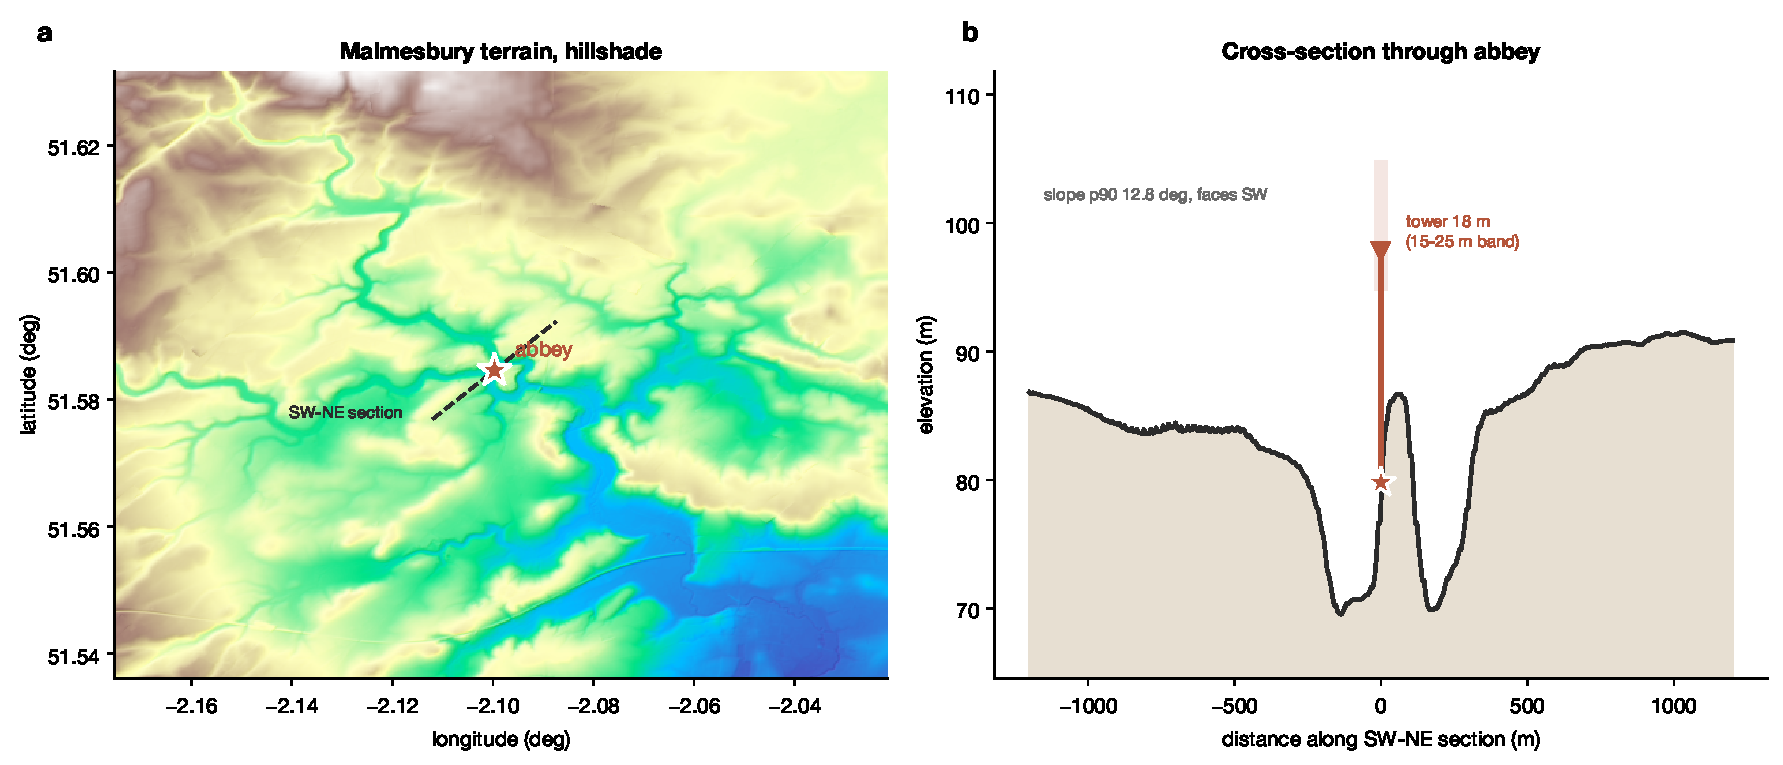
\includegraphics[width=\linewidth]{fig1_site}
  \caption{\textbf{Site and launch geometry at Malmesbury Abbey.}
  \textbf{(a)} Hillshaded terrain (AWS Terrain Tiles, about \SI{6}{\meter} posting)
  with the abbey on a promontory above the confluence of two Avon branches; the
  SW--NE line marks the section in (b).
  \textbf{(b)} Elevation along the section. The abbey stands \SI{10.2}{\meter} above
  the valley floor on a SW-facing slope (aspect \ang{230}; slope within
  \SI{400}{\meter}: mean \ang{5.2}, p90 \ang{12.8}).
  The \SI{6}{\meter} DEM under-resolves the launch edge, so the reported slope is a
  lower bound pending LIDAR.}
  \label{fig:site}
\end{figure}

\subsection{Favourable launch winds are common}

Over twenty years of ERA5 reanalysis, the wind blows from the SW sector at a
launchable \SIrange{5}{12}{\meter\per\second} in \SI{15.6}{\percent} of all hours
(\SI{95}{\percent} CI \numrange{14.3}{17.0}), about \num{1370} hours per year, with
a winter peak of \SI{21.1}{\percent} (\cref{fig:wind}).
The SW sector at any speed accounts for \SI{34.3}{\percent} of hours, so the
prevailing wind and the escarpment are well aligned.
A would-be flyer who waits for his conditions has them on the order of a thousand
hours a year, and the medieval wind regime appears no weaker than today's, so this
estimate is conservative for Eilmer's time.

\begin{figure}[htbp]
  \centering
  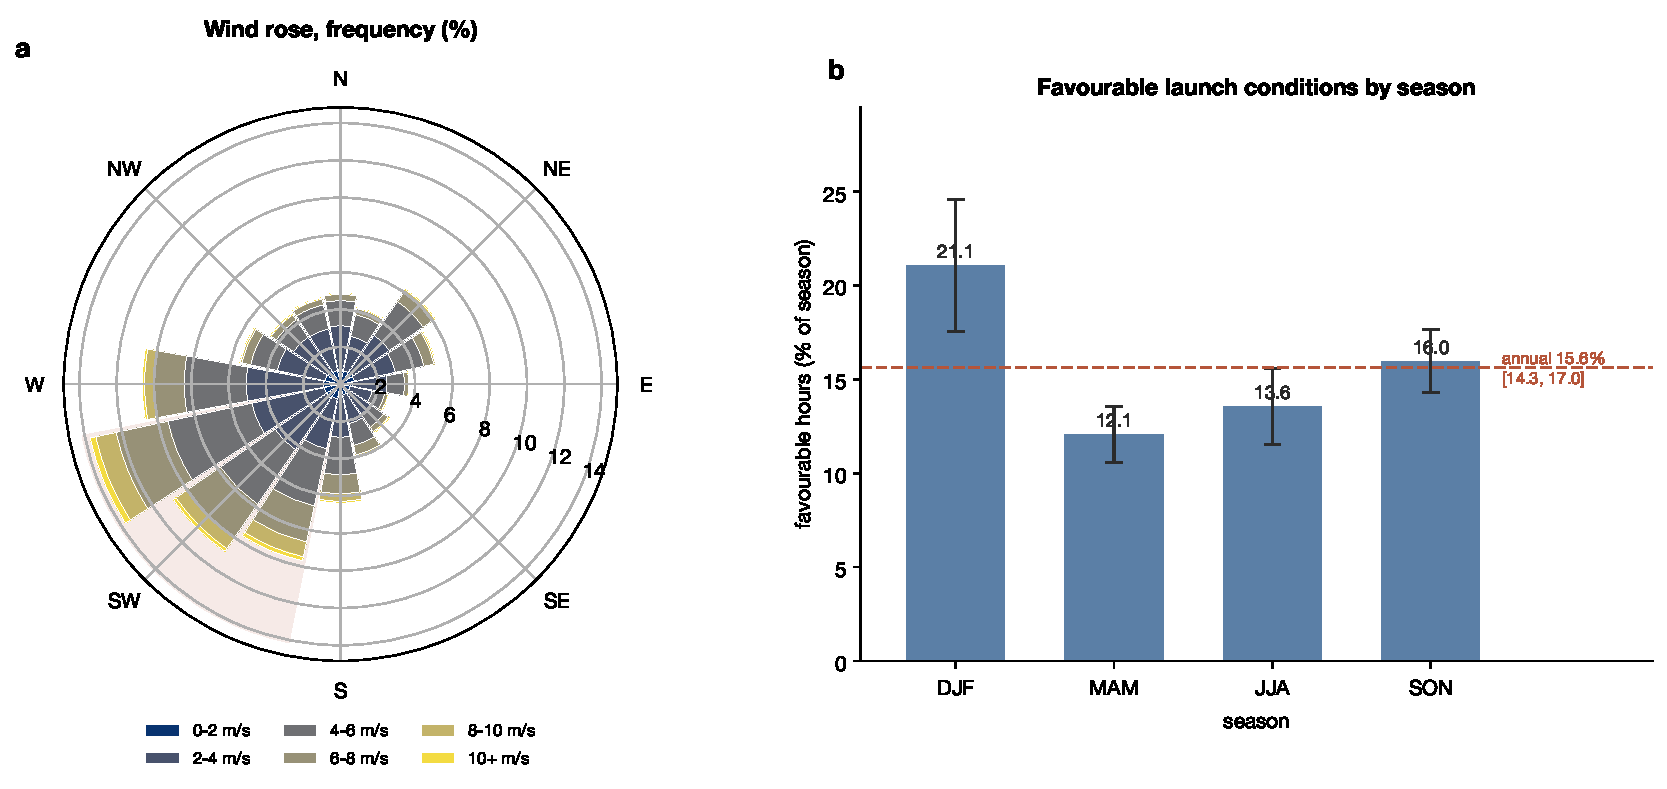
\includegraphics[width=\linewidth]{fig2_wind}
  \caption{\textbf{Favourable launch winds are common.}
  \textbf{(a)} Wind rose of ERA5 hourly \SI{10}{\meter} wind at the abbey,
  2004--2023 (\num{175320} hours).
  \textbf{(b)} Fraction of hours offering a favourable launch (SW sector
  \ang{191}--\ang{259} at \SIrange{5}{12}{\meter\per\second}), annually and by
  season, with \SI{95}{\percent} confidence intervals across the twenty years.
  Favourable conditions occur in \SI{15.6}{\percent} of hours (\SI{95}{\percent} CI
  \numrange{14.3}{17.0}), about \num{1370} hours per year, peaking in winter
  (\SI{21.1}{\percent}).}
  \label{fig:wind}
\end{figure}

\subsection{Ridge lift supplies the missing glide performance}

The linear orographic model (\cref{eq:ridge}) over the real terrain section gives a
peak upwash of about \SI{1.5}{\meter\per\second} just southwest of the abbey for an
\SI{8}{\meter\per\second} wind, with a soarable band about \SI{38}{\meter} deep
(\cref{fig:ridge}, supplementary).
That exceeds the optimistic sink of a crude glider
(\SIrange{0.75}{1.0}{\meter\per\second}), so the slope can in principle hold the
apparatus aloft, or at least flatten its descent, over the launch zone.
The mechanism is present and of the right order; with the smoothed DEM, both the
modelled slope and the lift it produces are lower bounds, which is why we keep the
full field in the supplement and carry only its magnitude into the glide analysis.

\subsection{A 200 m glide needs the wind}

In still air, covering \SI{200}{\meter} from an \SI{18}{\meter} tower demands a
glide ratio of \num{11.1}, which is sailplane class and far beyond a wood-and-cloth
wing (\cref{fig:glide}).
Adding the modelled ridge lift collapses the requirement: above
\SI{3.6}{\meter\per\second} of southwest wind the required glide ratio drops into
the crude cambered-wing band (\LD\ \numrange{3}{7}), reaching \num{4.8} at
\SI{8}{\meter\per\second}.
An \LD~5 wing launched into that wind clears \SI{200}{\meter} at about
\SI{7.5}{\meter\per\second}, inside the favourable band of \cref{fig:wind}.
The distance is achievable, but only with the wind and slope doing part of the work;
a calm-air leap from the tower would fall far short.

\begin{figure}[htbp]
  \centering
  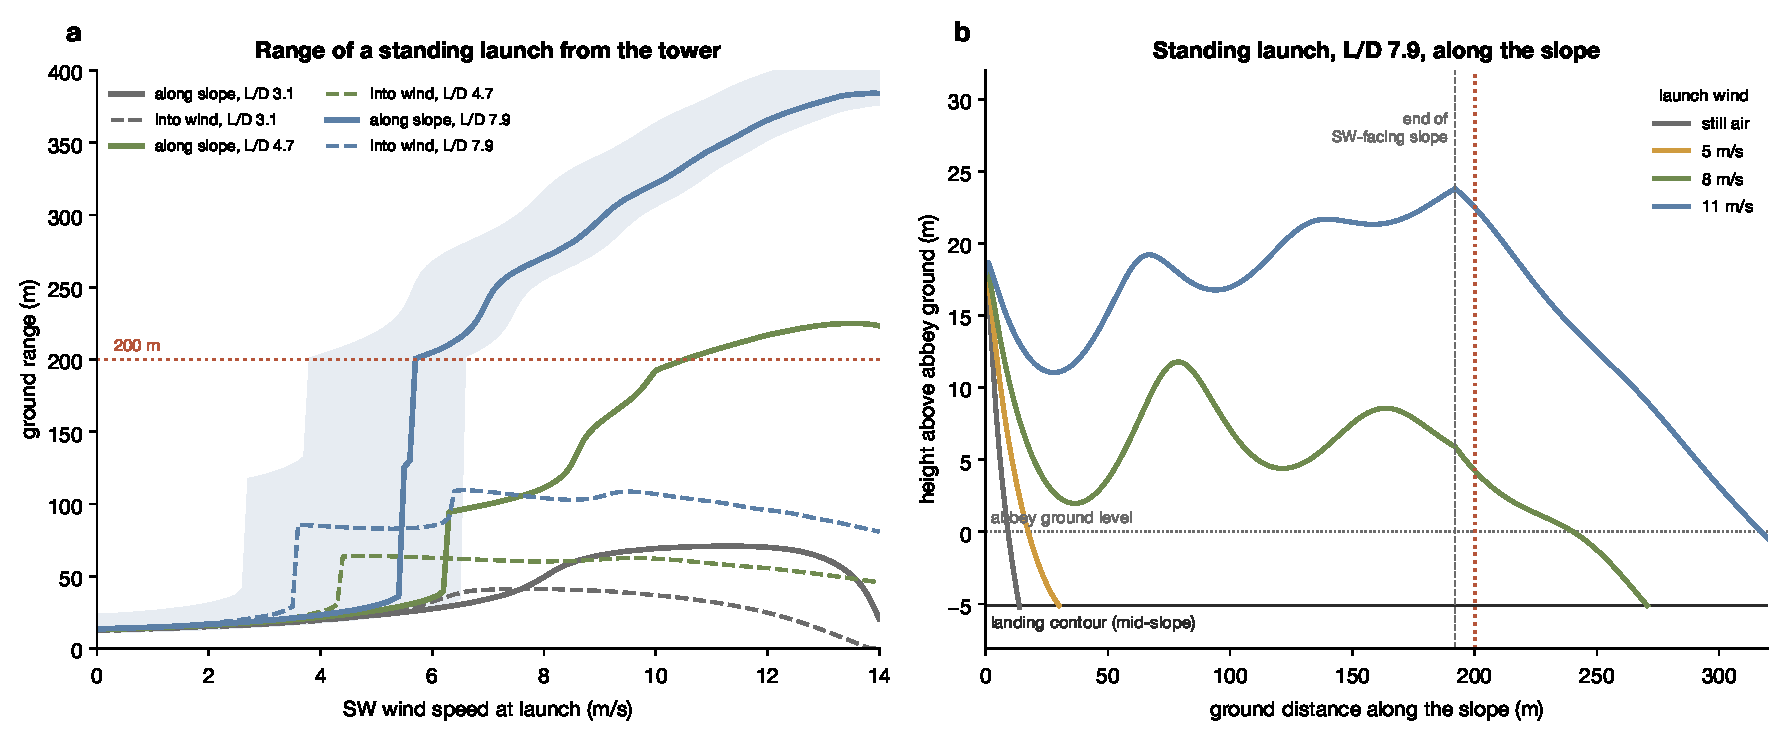
\includegraphics[width=\linewidth]{fig4_glide_envelope}
  \caption{\textbf{A \SI{200}{\meter} glide needs wind and slope.}
  \textbf{(a)} Range of an \LD~5 cambered wing launched from an \SI{18}{\meter}
  tower versus southwest wind speed; \SI{200}{\meter} is reached at about
  \SI{7.5}{\meter\per\second}.
  \textbf{(b)} Glide ratio required to cover \SI{200}{\meter} versus wind speed.
  Still air demands \LD~\num{11.1} (sailplane class, dotted line); with ridge lift
  the requirement falls into the crude cambered-wing band (\LD\ \numrange{3}{7})
  above \SI{3.6}{\meter\per\second}, reaching \LD~\num{4.8} at
  \SI{8}{\meter\per\second}.}
  \label{fig:glide}
\end{figure}

\subsection{The tailless craft cannot hold pitch}

A hanging pilot's CG (\numrange{0.35}{0.55}\,\(c\)) sits aft of a tailless wing's
neutral point (\(0.25\,c\)), so the configuration is statically unstable for every
posture the pilot can adopt (\cref{fig:stability}).
The instability is fast: after an \ang{8} gust the pitch attitude crosses the
\ang{60} loss-of-control threshold in \SI{0.74}{\second}, and the pitch error
doubles in \SIrange{0.1}{0.5}{\second} across the whole CG band, even with pitch
inertia varied by a factor of two, against a representative flight lasting
\SI{13.3}{\second}.
Fitting a tail moves the neutral point aft to \(0.53\,c\) and adds strong pitch
damping, which removes the divergence entirely.
The aerodynamics single out exactly the part Eilmer said he had left off.

\begin{figure}[htbp]
  \centering
  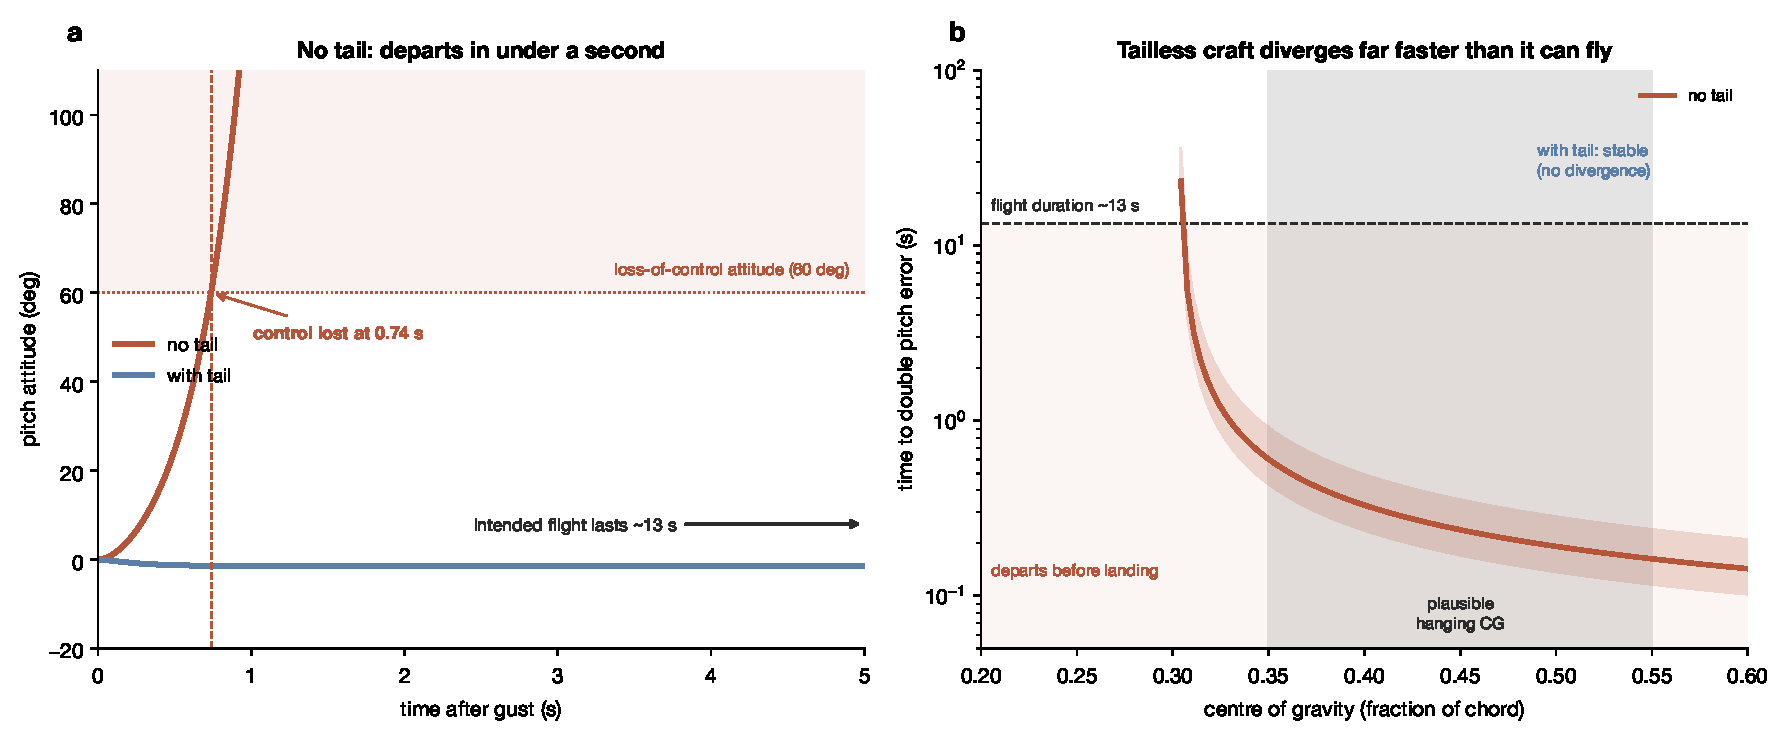
\includegraphics[width=\linewidth]{fig5_stability}
  \caption{\textbf{The tailless craft cannot hold pitch.}
  \textbf{(a)} Pitch-attitude response to an \ang{8} gust. Without a tail (red) the
  attitude crosses the \ang{60} loss-of-control line \SI{0.74}{\second} after the
  gust; with a tail (blue) the same gust damps out.
  \textbf{(b)} Time to double the pitch error across the plausible CG band:
  \SIrange{0.1}{0.5}{\second} everywhere for the tailless craft (pitch inertia
  varied \numrange{0.5}{2}\(\times\)), far shorter than the flight, and no
  divergence with a tail. A tail shifts the neutral point from \(0.25\,c\) to
  \(0.53\,c\), aft of a hanging pilot's CG (\numrange{0.35}{0.55}\,\(c\)).}
  \label{fig:stability}
\end{figure}

\subsection{The feasibility envelope}

Sampling the unknown apparatus and launch day \num{40000} times, \SI{27}{\percent}
of plausible worlds reach \SI{200}{\meter} (\SI{95}{\percent} CI \numrange{26}{27}),
with a median range of \SI{147}{\meter} (\cref{fig:montecarlo}a).
The typical draw falls short, but a furlong is far from rare, and Eilmer chose his
day and presumably his build, placing him in the upper tail.
Whether a reaching flight survives turns entirely on the tail, through a clean
timescale separation (\cref{fig:montecarlo}b): a tailless craft's pitch error
doubles in a median \SI{0.27}{\second} (p99 \SI{1.6}{\second}), with control lost
after about \SI{3}{\meter} of flight, while the glide must stay controlled for a
median \SI{20}{\second}, roughly \(75\times\) longer.
Every tailed configuration that reaches \SI{200}{\meter} is statically stable and
never diverges.
The model reproduces the reported sequence: he covered the distance, then lost
control.

\begin{figure}[htbp]
  \centering
  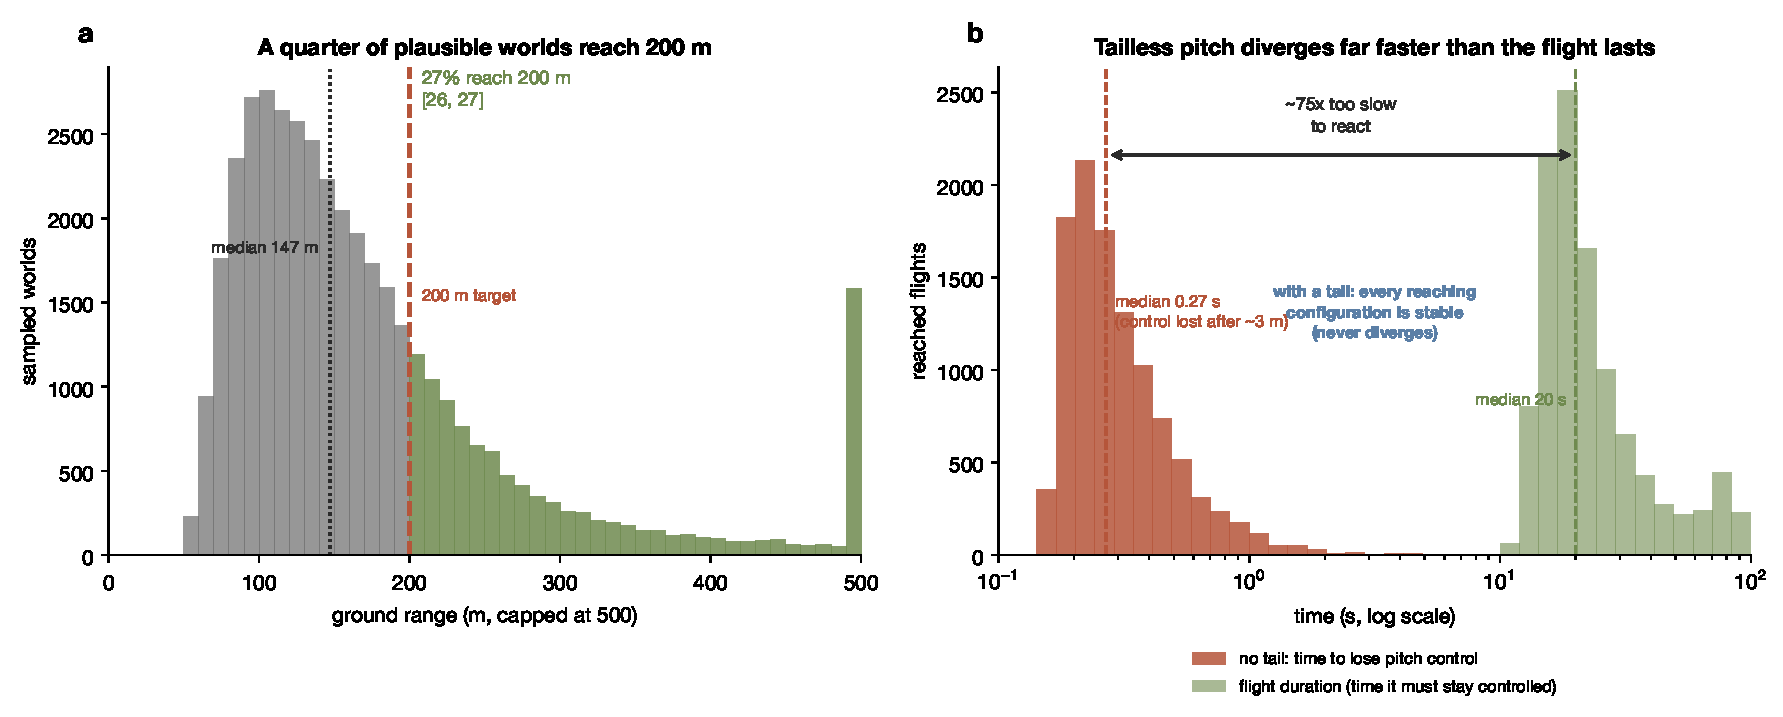
\includegraphics[width=\linewidth]{fig6_montecarlo}
  \caption{\textbf{Feasibility envelope over the unknown apparatus and day.}
  \num{40000} Monte Carlo samples drawing apparatus and launch parameters from
  plausible ranges, with launch wind drawn from the actual ERA5 SW-sector launchable
  speeds.
  \textbf{(a)} \SI{27}{\percent} of worlds reach \SI{200}{\meter} (\SI{95}{\percent}
  CI \numrange{26}{27}; median range \SI{147}{\meter}).
  \textbf{(b)} Among the reaching flights, tailless pitch error doubles in a median
  \SI{0.27}{\second} (p99 \SI{1.6}{\second}) against a flight that must stay
  controlled for a median \SI{20}{\second}, while tailed configurations never
  diverge.}
  \label{fig:montecarlo}
\end{figure}

\subsection{Broken legs fit an out-of-control arrival}

The reported injury is itself evidence (\cref{fig:biomech}).
A flared touchdown arrives at the sink rate (\SIrange{1}{3}{\meter\per\second}),
which is far below the tibia fracture-onset speed of about
\SI{9.7}{\meter\per\second} (range \numrange{7.5}{11.5}), so a controlled landing
could not break the legs.
An uncontrolled departure arrives near flying speed, with a vertical component of
\(V\sin\theta\), and breaks both tibiae with probability \num{0.66}, yet at about
\num{28}\,g over the legs it stays within the survivable feet-first regime rather
than the fatal one.
The injuries are thus positive evidence that Eilmer arrived out of control, the same
failure mode the missing tail predicts in \cref{fig:stability,fig:montecarlo}.

\begin{figure}[htbp]
  \centering
  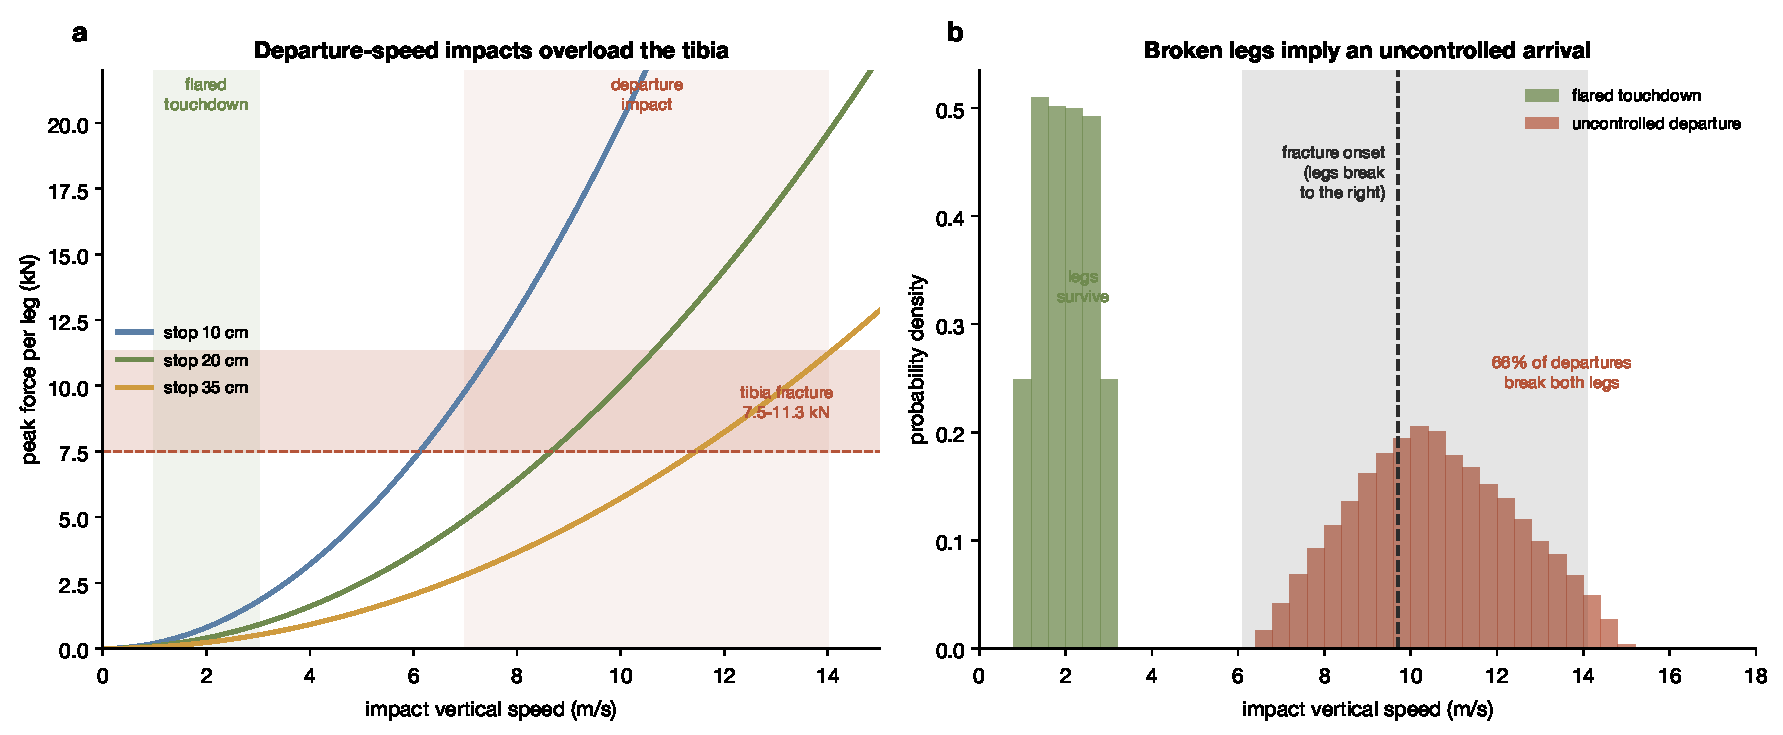
\includegraphics[width=\linewidth]{fig7_biomech}
  \caption{\textbf{Broken legs as evidence of an out-of-control arrival.}
  \textbf{(a)} Average feet-first impact force per leg versus vertical impact speed
  for ground-give distances \(d = \SIrange{10}{35}{\centi\meter}\), against the axial
  tibia fracture band (\SIrange{7.5}{11.3}{\kilo\newton} per leg). Fracture onset is
  about \SI{9.7}{\meter\per\second}.
  \textbf{(b)} Impact-speed distributions for a flared touchdown
  (\SIrange{1}{3}{\meter\per\second}) versus an uncontrolled departure
  (\(V\sin\theta\), \(V=\SIrange{11}{16}{\meter\per\second}\),
  \(\theta=\ang{35}\)--\ang{70}). A departure breaks both tibiae with probability
  \num{0.66} yet, at about \num{28}\,g, remains survivable.}
  \label{fig:biomech}
\end{figure}
\FloatBarrier

\section{Discussion}

The account survives every test we can pose.
The site geometry, the wind climatology, the glide physics, the pitch stability, and
the impact biomechanics line up with what William reports, and they converge on the
same cause of failure that Eilmer himself named.
Some of these results hold regardless of our modelling choices and some depend on
them, and the two should not be read with equal confidence.

What holds firm does not depend on the fine detail of the apparatus.
The escarpment faces the prevailing wind and favourable launch conditions are common
(\cref{fig:site,fig:wind}); this is measured, not modelled.
The static instability of a tailless hand-and-foot wing is similarly hard to escape:
it follows from the pilot's CG lying aft of the wing's neutral point, which holds for
every posture and every plausible wing in the Monte Carlo
(\cref{fig:stability,fig:montecarlo}).
And the qualitative biomechanics are one-directional: a gentle landing cannot break
two legs, so the injury implies speed at impact (\cref{fig:biomech}).

What is model-dependent is the quantitative margin.
The ridge-lift magnitude rests on a first-order linear model over a smoothed
\SI{6}{\meter} DEM (\cref{eq:ridge}), so the \SI{1.5}{\meter\per\second} upwash and
the \SI{3.6}{\meter\per\second} wind threshold are order-of-magnitude statements that
a LIDAR-resolved large-eddy solve should sharpen.
The \SI{27}{\percent} reach fraction is a function of the priors we placed on wing
area, mass, and glide ratio, and should be read as the spread of a plausible space
rather than a calibrated probability.
The stability analysis is a linear short-period treatment of the pitch axis alone;
the lateral modes and the nonlinear post-departure motion need a full six-degree-of
freedom model before the \(75\times\) timescale separation can be called exact.

The Ibn Firnas parallel deserves a closer look in light of these results.
If two of the earliest credible glide attempts both ended in a tailless
loss-of-control arrival \autocite{anderson2024bridge}, the convergence is not
coincidence but physics: a tail is the one component an untutored builder is most
likely to omit and the one whose absence most reliably ends the flight.
The method here, terrain plus climate plus first-principles flight dynamics, can be
pointed at that account and others on the same footing.

The main threats to the conclusion are the unknown apparatus and the coarse terrain.
We mitigate the first with the Monte Carlo and the second by reporting slope and
lift as lower bounds, but neither is a substitute for the two obvious next steps: an
airborne-LIDAR terrain model with a microscale wind solve, and a structural analysis
of a willow-and-cloth wing under the computed flight loads to rule out a structural,
rather than control, failure.
We also do not reconstruct the actual flight.
We show that the reported flight is physically consistent and that its stated cause
is correct, which is a different and more defensible claim than asserting it happened
exactly as written.

\section{Conclusion}

William of Malmesbury's account of Eilmer's flight is aerodynamically
self-consistent.
A wind-and-slope-assisted glide of about \SI{200}{\meter} from the abbey is feasible
for a crude cambered wing, the tailless configuration Eilmer blamed would by itself
cause loss of pitch control within a second of a disturbance, and the broken legs he
suffered fit the predicted out-of-control impact while remaining survivable.
The monk's own diagnosis, that he should have fitted a tail, is correct.

We do not claim the flight happened exactly as written, and the quantitative margins
depend on a coarse terrain model and a first-order lift model that airborne LIDAR and
a microscale wind solve would sharpen.
What we provide is a calibrated verdict on a specific eleventh-century claim and a
reproducible pipeline, from terrain and climate to flight dynamics and biomechanics,
for adjudicating pre-modern flight accounts.
The same method applied to Ibn Firnas and the other early gliding reports would test
whether the want of a tail is the recurring cause it appears to be.

\section*{Data and code availability}

The full analysis pipeline, raw data manifests, and figure-generation scripts
rebuild every number and figure in this paper from one driver script. They are
openly available at \url{https://github.com/silverdavi/eilmer-flight-feasibility}
and archived at \url{https://doi.org/10.5281/zenodo.20706321}.

\section*{Acknowledgements}

We thank the Athelstan Museum, Malmesbury, for curating the local record of Eilmer's
flight.


\printbibliography

\clearpage
\setcounter{figure}{0}
\setcounter{table}{0}
\renewcommand{\thefigure}{S\arabic{figure}}
\renewcommand{\thetable}{S\arabic{table}}
\section*{Supplementary material}
\addcontentsline{toc}{section}{Supplementary material}

\subsection*{S1. Verbatim source extracts for load-bearing claims}

Three claims carry the argument: the primary account of the flight, the tibia
fracture threshold behind the biomechanics, and the medieval wind regime behind the
climatology. We quote each source directly so the reader can check our reading.

\paragraph{S1.1 The flight, the distance, the injury, and the tail.}
The entire factual basis is one passage of William of Malmesbury, \textit{Gesta
Regum Anglorum} (book II, ch. 225), in the Oxford Medieval Texts edition
\autocite{williamMalmesbury_gesta}. The Latin reads:

\begin{quote}\small\itshape
Is erat litteris, quantum ad id temporis, bene imbutus, aeuo maturus, immanem
audaciam prima iuuentute conatus: nam pennas manibus et pedibus haud scio qua
innexuerat arte, ut Daedali more uolaret, fabulam pro uero amplexus, collectaque e
summo turris aura, spatio stadii et plus uolauit; sed uenti et turbinis uiolentia,
simul et temerarii facti conscientia, tremulus cecidit, perpetuo post haec debilis,
et crura effractus. Ipse ferebat causam ruinae quod caudam in posteriori parte
oblitus fuerit.
\end{quote}

\noindent In the standard English rendering:

\begin{quote}\small
He had by some means, I scarcely know what, fastened wings to his hands and feet so
that, mistaking fable for truth, he might fly like Daedalus, and, collecting the
breeze on the summit of a tower, he flew for more than the distance of a furlong.
But, agitated by the violence of the wind and the swirling of air, as well as by
awareness of his rashness, he fell, broke his legs, and was lame ever after. He
himself used to say that the cause of his failure was his forgetting to put a tail
on the back part.
\end{quote}

\noindent Every element we model is in these two sentences: the tower launch, the
hand-and-foot wings, the breeze, the furlong (a stadium, about \SI{200}{\meter}),
the loss of control in gusty air, the broken legs and permanent lameness, and the
diagnosis (\textit{caudam \ldots oblitus}, ``forgetting a tail'').

\paragraph{S1.2 The tibia fracture threshold.}
The \SIrange{7.5}{11.3}{\kilo\newton} per-leg band in \cref{fig:biomech} comes from
the injury-biomechanics literature, consolidated in a recent systematic review
\autocite{abidin2026tibia}, which reports that

\begin{quote}\small
tibial fracture thresholds range from \(\sim\)7.5 kN in female specimens to 11.3 kN
under combined axial and bending loads, with fibula contribution increasing axial
tolerance by \(\sim\)10\%.
\end{quote}

\noindent The upper figure traces to the primary compilation of
\textcite{salzar2014leg}, which recommends a tibial axial threshold of
\(\sim\)\SI{10.3}{\kilo\newton} rising to \(\sim\)\SI{11.3}{\kilo\newton} with the
fibula's contribution. We use the range, not a point value, precisely because the
threshold depends on sex, loading rate, and bending.

\paragraph{S1.3 The medieval wind regime.}
The claim that modern reanalysis is a reasonable, probably conservative proxy for
Eilmer's epoch rests on reconstructions of the North Atlantic Oscillation, which
disagree on timing. \textcite{trouet2009nao} report

\begin{quote}\small
a 947-year-long multidecadal North Atlantic Oscillation (NAO) reconstruction [with]
a persistent positive NAO during the MCA [Medieval Climate Anomaly].
\end{quote}

\noindent The later, model-tested reconstruction of \textcite{ortega2015nao}
revises this, finding

\begin{quote}\small
no persistent positive NAO during the medieval period, but [suggesting] that
positive phases were dominant during the thirteenth and fourteenth centuries.
\end{quote}

\noindent We therefore make only the weaker claim the evidence supports: neither
reconstruction indicates the weak westerlies of a negative NAO over Britain in
Eilmer's period, so the favourable-wind fraction we compute from 2004--2023 ERA5
(\cref{fig:wind}) is not an overestimate for the eleventh century. We do not rely on
medieval winds being \emph{stronger} than modern ones.

\subsection*{S2. Monte Carlo parameter priors}

\Cref{tab:priors} lists the plausible ranges sampled in the feasibility envelope
(\cref{fig:montecarlo}). All priors are uniform over the stated range.

\begin{table}[htbp]
  \centering
  \caption{\textbf{Sampled parameter ranges for the Monte Carlo
  (\cref{fig:montecarlo}).} Launch wind is not sampled from a prior but drawn from
  the empirical ERA5 SW-sector launchable speeds (\cref{fig:wind}).}
  \label{tab:priors}
  \small
  \begin{tabular}{lll}
    \toprule
    Parameter & Range & Basis \\
    \midrule
    Wing area & \SIrange{5}{10}{\meter\squared} & crude hand/foot wing \\
    All-up mass & \SIrange{70}{90}{\kilogram} & adult pilot plus apparatus \\
    Trim \(C_L\) & \numrange{0.7}{1.1} & cambered cloth, low Reynolds number \\
    Glide ratio \LD & \numrange{3}{7} & hang-glider class, crude build \\
    Tower height & \SIrange{15}{25}{\meter} & abbey tower, conservative \\
    Escarpment slope & \ang{8}--\ang{18} & DEM p90 as a floor \\
    Ridge-lift efficiency & \numrange{0.5}{1.0} & attached-upslope fraction \\
    Centre of gravity & \numrange{0.35}{0.55}\,\(c\) & hanging-pilot range \\
    Aspect ratio & \numrange{3}{5} & span/area of a hand-foot wing \\
    Tail neutral-point shift & \numrange{0.18}{0.32}\,\(c\) & tail size variation \\
    \bottomrule
  \end{tabular}
\end{table}

\subsection*{S3. Ridge-lift field}

\Cref{fig:ridge} shows the first-order orographic lift field summarised in the main
text. We keep the full field here because the smoothed \SI{6}{\meter} DEM makes the
modelled slope, and therefore the lift, a lower bound; the main analysis carries
only its magnitude.

\begin{figure}[htbp]
  \centering
  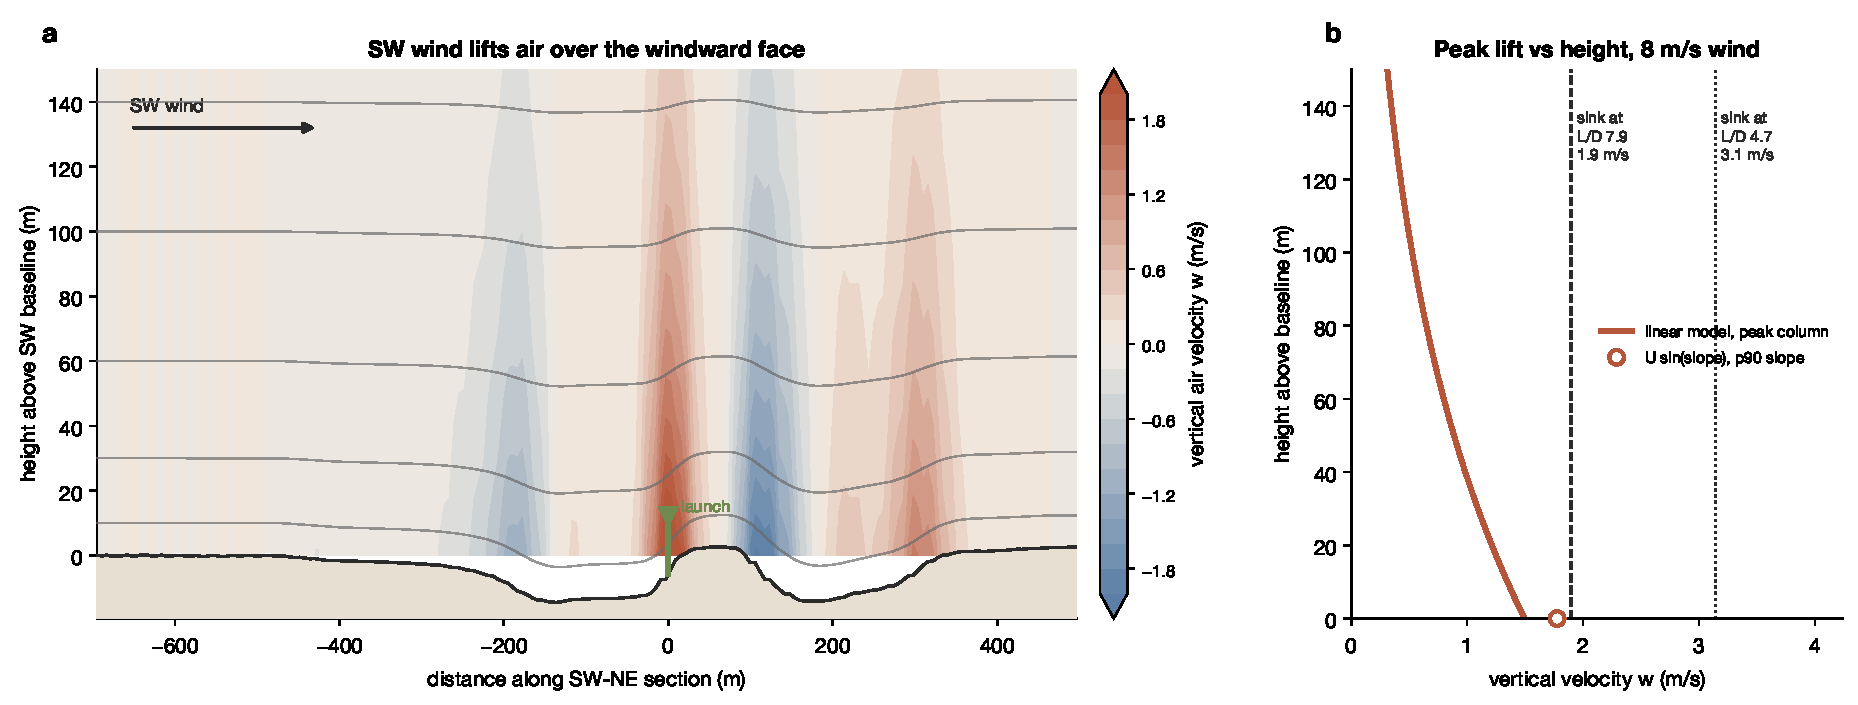
\includegraphics[width=\linewidth]{fig3_ridge_lift}
  \caption{\textbf{Ridge lift over the escarpment matches a crude glider's sink.}
  A first-order linear orographic model (\(w = U\,\mathrm{d}h/\mathrm{d}x\,e^{-kz}\))
  over the real SW--NE terrain section.
  \textbf{(a)} Vertical-velocity field and streamlines for an
  \SI{8}{\meter\per\second} southwest wind.
  \textbf{(b)} Lift versus height above the windward face. Peak lift just southwest
  of the abbey is about \SI{1.5}{\meter\per\second}, above a crude glider's
  optimistic sink of \SIrange{0.75}{1.0}{\meter\per\second}, with a soarable band
  about \SI{38}{\meter} deep.}
  \label{fig:ridge}
\end{figure}


\end{document}
